\documentclass{article}

\usepackage[final]{neurips_2025}

\usepackage[T1]{fontenc}
\usepackage[utf8]{inputenc}
\usepackage{hyperref}
\usepackage{url}
\usepackage{booktabs}
\usepackage{amsfonts}
\usepackage{nicefrac}
\usepackage{microtype}
\usepackage{xcolor}
\usepackage{graphicx}
\usepackage{amsmath,amssymb}
\usepackage{subcaption}

\title{GFlowNet-Guided Dropout Mask Sampling for Neural Bayesian Optimization}
\author{Anuar Aimoldin}
\date{}

\begin{document}
\maketitle

\begin{abstract}
This project studies whether learned dropout-mask generation improves neural Bayesian optimization over random mask sampling. The proposed method trains a contextual sequential GFlowNet to sample block-wise dropout masks using a proxy improvement reward, while the baseline samples masks uniformly at random. To improve internal validity, all final experiments use a controlled evaluation protocol with matched per-step candidate pools, aligned training and inference mask semantics, and explicit reward-reliability diagnostics. Across Branin (2D), Hartmann-6 (6D), and Ackley-10 (10D), the empirical result is mixed: random masks perform better on Branin and Hartmann-6, while the GFlowNet policy achieves lower final regret on Ackley-10. Within this benchmark configuration, the evidence suggests a conditional, benchmark-dependent benefit rather than universal improvement.
\end{abstract}

\section{Introduction}

Bayesian optimization (BO) is a standard framework for optimizing expensive black-box objectives under a limited evaluation budget \cite{snoek2012practical}. Classical BO uses a probabilistic surrogate, often a Gaussian process, together with an acquisition function that balances exploration and exploitation. In this project, I study a neural alternative in which the surrogate is a dropout MLP and uncertainty is represented through stochastic masked forward passes, following the Bayesian interpretation of dropout from \citet{gal2016dropout}.

The main question is whether mask sampling itself can be made more informative. Instead of treating dropout masks as undirected random perturbations, I model mask generation as a structured sampling problem and learn a distribution over masks with a GFlowNet \cite{bengio2023gflownet}. Recent work on GFlowOut shows that GFlowNets can represent useful distributions over dropout masks in supervised learning \cite{liu2023gflowout}; here I test the same idea inside a BO loop. This study compares learned mask generation against a matched random MC-Dropout baseline on standard BO benchmarks, uses contextual conditioning to study non-stationarity as the surrogate evolves, and reports the regret-versus-compute trade-off rather than regret alone.

This study is a controlled proof-of-concept. Its goal is to test whether learned dropout-mask generation yields a reproducible advantage over random MC-Dropout under a standardized evaluation protocol.

The contributions of this report are threefold: (1) a contextual GFlowNet formulation for sequential dropout-mask generation inside a neural BO loop; (2) a controlled and reproducible benchmark protocol with matched within-step evaluation contexts and explicit reward diagnostics; and (3) an empirical study showing that the resulting benefit is benchmark-dependent and currently comes with substantial computational overhead.

\section{Research Questions}

This study focuses on four questions:

\begin{enumerate}
    \item Can learned mask generation outperform random mask sampling for BO exploration?
    \item Are gains more visible on Ackley-10 within the current benchmark suite, and to what extent can that be separated from dimensionality?
    \item How should the mask policy adapt as the dataset and surrogate change over BO iterations?
    \item Is the extra compute required for GFlowNet training justified by lower regret?
\end{enumerate}

\section{Method}

\subsection{Masked Neural Surrogate}

At BO iteration $t$, the observed dataset is
\[
\mathcal{D}_t = \{(x_i, y_i)\}_{i=1}^{n_t}, \qquad y_i = f(x_i).
\]

The surrogate is a two-hidden-layer MLP trained on normalized inputs and targets. Each hidden layer has dropout during training. At inference time, instead of sampling element-wise dropout, I use a \emph{block-wise} binary mask $m \in \{0,1\}^B$ that deterministically keeps or removes contiguous hidden blocks. A mask defines a masked predictor $\hat f_\theta(x; m)$.

\subsection{Proposal Generation from a Mask}

Given a finite candidate set $\mathcal{C}_t$, each mask induces a proposed point
\[
x_m = \arg\max_{x \in \mathcal{C}_t} \hat f_\theta(x; m).
\]

To estimate whether the proposal is promising, I evaluate $x_m$ under a held-out ensemble of random masks $h_1,\dots,h_H$. This produces a proxy mean and standard deviation,
\[
\tilde\mu(x_m) = \frac{1}{H}\sum_{j=1}^H \hat f_\theta(x_m; h_j),
\qquad
\tilde\sigma(x_m) = \mathrm{Std}\big[\hat f_\theta(x_m; h_j)\big].
\]

Let $y_t^{\mathrm{best}}$ be the best observed oracle value so far. The proxy improvement score is
\[
\Delta(m) = \tilde\mu(x_m) + \beta \tilde\sigma(x_m) - y_t^{\mathrm{best}},
\]
which is then converted into a positive reward $R(m)$ used for mask sampling. The ideal reward in the project formulation depends on realized oracle improvement, but using that quantity online would require additional expensive objective evaluations. I therefore optimize a surrogate-based proxy reward computed from held-out masked evaluations. This is not merely a practical shortcut; it is one of the central approximations of the method. For that reason, reward reliability is treated as a first-class diagnostic target alongside regret. In the original implementation this conversion used a fixed softplus transform. In the final controlled pipeline, reward scaling is treated as an explicit protocol choice, with raw, normalized, and rank-based variants available as controlled alternatives. Across all variants, the underlying objective is the same: reward masks that both predict high value and preserve some uncertainty through the held-out ensemble.

\subsection{Random Baseline vs. GFlowNet Policy}

The two compared policies differ only in how masks are generated:

\begin{itemize}
    \item \textbf{Random baseline:} sample block-wise masks uniformly at random, evaluate each sampled mask with $R(m)$, and query the proposal from the best mask in the sampled set.
    \item \textbf{GFN policy:} train a sequential GFlowNet so that $P(m \mid c_t) \propto R(m)$, then draw candidate masks from this learned policy and again query the proposal from the best sampled mask.
\end{itemize}

The GFlowNet generates masks one block at a time and is conditioned on a context vector $c_t$ computed from the current dataset. In the implementation, $c_t$ contains BO progress, normalized response statistics, input dispersion, and the benchmark dimension. This is a simple way to address non-stationarity as the BO loop evolves.

\section{Experimental Setup}

I evaluate the method on the three baselines requested in the project prompt:

\begin{itemize}
    \item Branin (2D), converted to maximization by optimizing $-\mathrm{Branin}(x)$,
    \item Hartmann-6 (6D),
    \item Ackley (10D), converted to maximization by optimizing $-\mathrm{Ackley}(x)$.
\end{itemize}

The main metric is simple regret,
\[
r_t = f^\star - \max_{i \le t} f(x_i),
\]
where $f^\star$ is the known benchmark optimum. Each experiment is run over 5 random seeds.

\begin{table}[t]
\centering
\caption{Benchmark-specific BO configurations used in the executed config-driven runs.}
\label{tab:configs}
\small
\begin{tabular}{lcccccc}
\toprule
Benchmark & Dim & $n_{\text{init}}$ & BO iters & Hidden dim & Candidate pool & GFN steps \\
\midrule
Branin & 2 & 8 & 18 & 64 & 2048 & 160 \\
Hartmann-6 & 6 & 14 & 22 & 96 & 4096 & 180 \\
Ackley & 10 & 20 & 24 & 128 & 4096 & 200 \\
\bottomrule
\end{tabular}
\end{table}

Across all benchmarks, each BO step compares 96 sampled masks for the random policy and 96 sampled masks for the GFlowNet policy. The proxy reward uses 24 held-out random masks. All experiments were executed in the \texttt{general\_env} conda environment. The final package is reproducibility-oriented: runs are config-driven, benchmark settings are fixed per task, candidate pools and held-out ensembles are shared within each BO step, and diagnostics are logged together with regret and runtime.

All main comparisons are budget-matched: both methods use the same surrogate architecture, BO horizon, number of sampled masks per step, and candidate-pool size. In addition, all mask evaluations within a BO step are performed under the same candidate pool and the same held-out mask ensemble, so the comparison isolates the mask-sampling policy rather than random variation in the evaluation context.

\subsection{Controlled Evaluation Protocol}

A substantial part of the project effort went into reducing ambiguity about whether the observed performance differences came from the method itself or from the surrounding evaluation protocol. The final \texttt{pkg} pipeline therefore introduces three controls that are important for interpreting the results.

First, all mask evaluations within a BO step now share the same candidate pool and the same held-out mask ensemble. This removes a major source of evaluation noise present in a naive implementation, where each mask could otherwise be scored against a different randomly drawn context. Second, the final pipeline aligns surrogate-side masking and policy-side search, removing a train/inference mismatch present in earlier prototypes. Third, the pipeline logs reward reliability diagnostics in addition to regret: step-wise reward variance, improvement variance, floor-reward frequency, same-mask repeat-evaluation variance, and the correlation between proxy improvement and realized oracle gain.

These controls do not guarantee that the proxy reward is perfectly calibrated, but they make the resulting conclusions more defensible. In particular, if a mixed or negative result persists after these implementation changes, it is less plausible to dismiss it as a simple artifact of noisy reward evaluation or an avoidable mismatch between training and inference.

\section{Results}

\begin{table}[t]
\centering
\caption{Final performance over 5 seeds. Lower regret is better.}
\label{tab:final_results}
\small
\begin{tabular}{lccc}
\toprule
Benchmark & Random final regret & GFlowNet final regret & Better method \\
\midrule
Branin (2D) & $1.7813 \pm 1.1734$ & $2.1459 \pm 0.7910$ & Random \\
Hartmann-6 (6D) & $0.5571 \pm 0.3059$ & $0.7027 \pm 0.5144$ & Random \\
Ackley (10D) & $18.1526 \pm 1.1661$ & $16.7447 \pm 1.5421$ & GFlowNet \\
\bottomrule
\end{tabular}
\end{table}

Table~\ref{tab:final_results} shows a clear mixed pattern. On the lower-dimensional benchmarks, learned mask generation did not outperform the random baseline. On Branin, the random policy finished with a lower mean regret by $0.3646$, which corresponds to the GFlowNet method performing about $20.5\%$ worse relative to the random baseline. On Hartmann-6, the gap in favor of random masks was smaller, $0.1456$, but it still corresponds to the GFlowNet method performing about $26.1\%$ worse. Ackley-10 was different: here the GFlowNet policy improved final regret by $1.4079$, or about $7.8\%$ relative to the random baseline, providing the strongest positive evidence for the method.

The controlled protocol did not change the benchmark-level conclusion.

\begin{figure*}[t]
    \centering
    \begin{subfigure}[t]{0.32\textwidth}
        \centering
        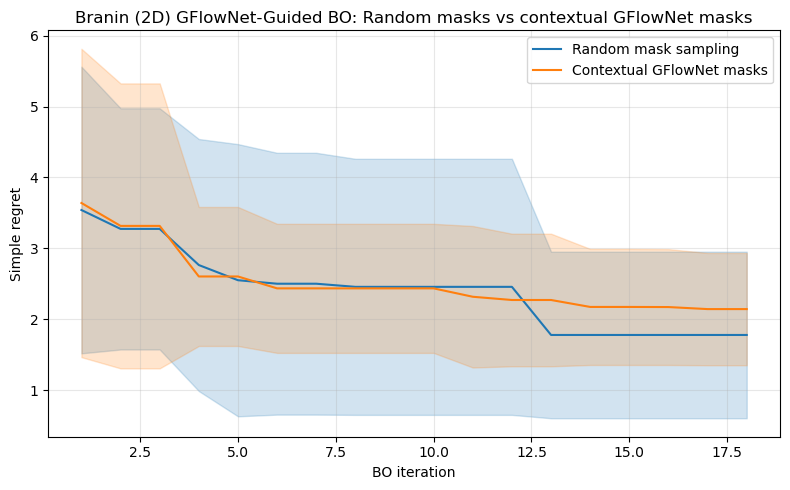
\includegraphics[width=\textwidth]{img/branin_regret_comparison.png}
        \caption{Branin (2D)}
    \end{subfigure}
    \hfill
    \begin{subfigure}[t]{0.32\textwidth}
        \centering
        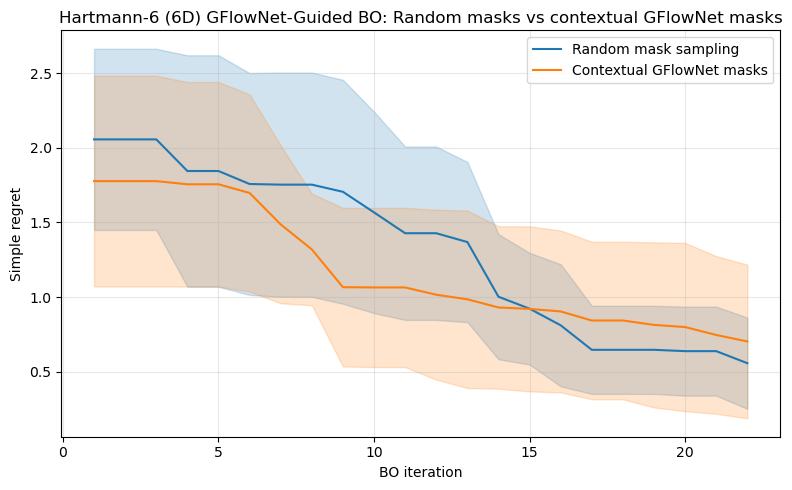
\includegraphics[width=\textwidth]{img/hartmann6_regret_comparison.png}
        \caption{Hartmann-6 (6D)}
    \end{subfigure}
    \hfill
    \begin{subfigure}[t]{0.32\textwidth}
        \centering
        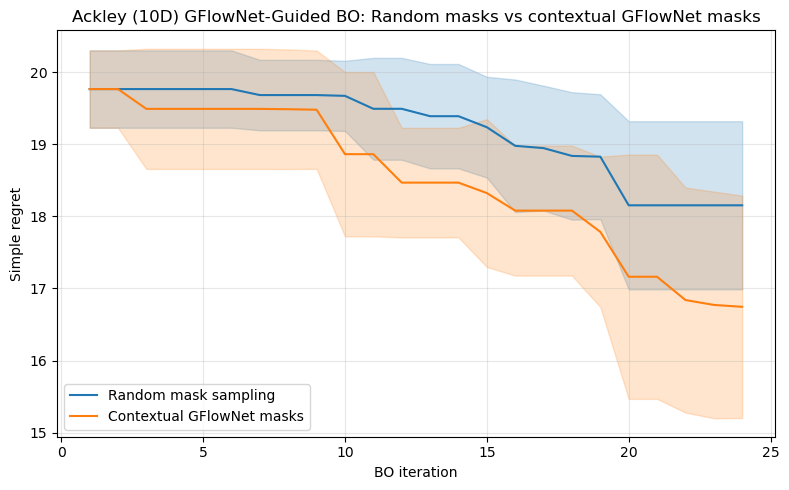
\includegraphics[width=\textwidth]{img/ackley10_regret_comparison.png}
        \caption{Ackley (10D)}
    \end{subfigure}
    \caption{Mean simple regret over BO iterations. Shaded regions denote one standard deviation across 5 seeds. Random mask sampling is stronger on Branin and Hartmann-6, while the contextual GFlowNet policy is stronger on Ackley-10.}
    \label{fig:regret_comparisons}
\end{figure*}

Figure~\ref{fig:regret_comparisons} makes the trend visible over the full optimization horizon. On Branin and Hartmann-6, the random baseline remains competitive throughout the run. On Ackley-10, the GFlowNet curve overtakes the random baseline and ends at a lower regret, suggesting that learned mask generation may be more useful in this benchmark configuration. Because the study uses only five seeds per benchmark, these quantities should be interpreted primarily as effect-size estimates rather than as definitive significance claims. Under that lens, the results indicate that the method is beneficial in some settings but not uniformly across benchmarks.

\begin{figure*}[t]
    \centering
    \begin{subfigure}[t]{0.48\textwidth}
        \centering
        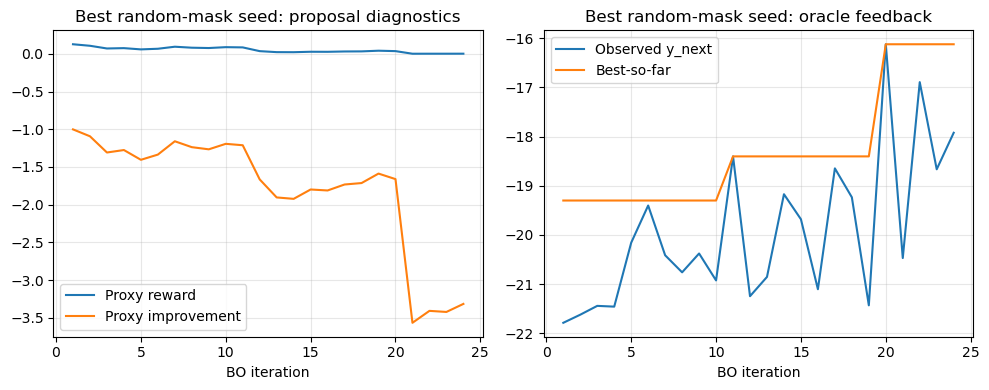
\includegraphics[width=\textwidth]{img/ackley10_random_diagnostics.png}
        \caption{Best random-mask seed on Ackley-10}
    \end{subfigure}
    \hfill
    \begin{subfigure}[t]{0.48\textwidth}
        \centering
        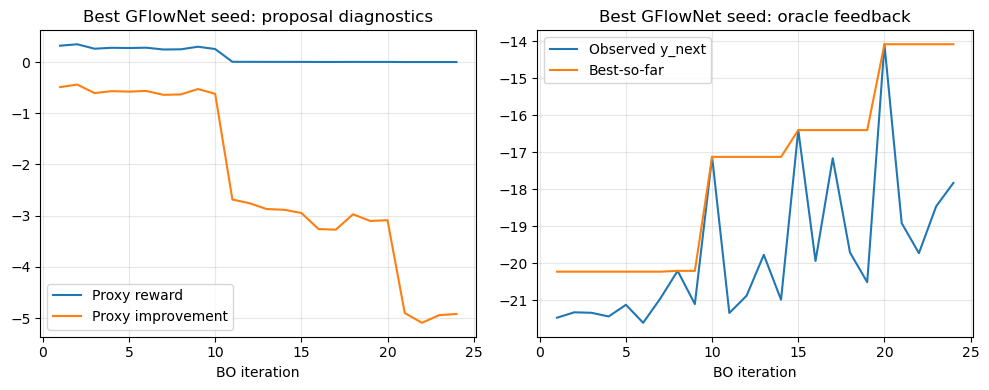
\includegraphics[width=\textwidth]{img/ackley10_gfn_diagnostics.png}
        \caption{Best GFlowNet seed on Ackley-10}
    \end{subfigure}
    \caption{Proposal diagnostics for Ackley-10. Each plot shows proxy reward and proxy improvement together with the actual queried oracle value and best-so-far trajectory. The GFlowNet run achieves stronger final best-so-far performance, which matches the lower final regret reported in Table~\ref{tab:final_results}.}
    \label{fig:ackley_diagnostics}
\end{figure*}

Figure~\ref{fig:ackley_diagnostics} shows that the best GFlowNet seed converts high proxy scores into a stronger best-so-far trajectory than the best random baseline seed on Ackley-10.

\subsection{Compute Trade-off}

Because GFlowNet-guided BO adds a learned mask-policy training loop inside each BO iteration, the wall-clock overhead is an important part of the result rather than an implementation detail. I therefore ran a separate timing experiment with the same benchmark configurations and seeds used for the main results. Table~\ref{tab:compute_tradeoff} compares mean final regret with mean wall-clock time per trial.

\begin{table}[t]
\centering
\caption{Compute trade-off over 5 seeds. Positive regret gain means GFlowNet achieved lower regret than the random baseline.}
\label{tab:compute_tradeoff}
\small
\begin{tabular}{lcccccc}
\toprule
Benchmark & Random regret & GFN regret & Random time & GFN time & Slowdown & Regret gain \\
\midrule
Branin & $1.7813$ & $2.1459$ & $3.75$s & $128.07$s & $34.11\times$ & $-0.3646$ \\
Hartmann-6 & $0.5571$ & $0.7027$ & $5.77$s & $310.73$s & $53.85\times$ & $-0.1456$ \\
Ackley & $18.1526$ & $16.7447$ & $7.52$s & $509.42$s & $67.70\times$ & $1.4079$ \\
\bottomrule
\end{tabular}
\end{table}

The compute trade-off is severe. On Branin and Hartmann-6, the GFlowNet policy is both slower and worse. In those settings, the extra computation is clearly not justified. Ackley-10 is the only benchmark where the additional training cost buys a measurable optimization benefit: GFlowNet improves mean final regret by $1.4079$, but it does so while increasing mean wall-clock time per trial from $7.52$ seconds to $509.42$ seconds. The compute overhead is substantial, and its practical value is clearest only on Ackley-10.

\begin{table}[t]
\centering
\caption{Mean per-iteration runtime breakdown in seconds. The dominant extra cost comes from GFlowNet training, not surrogate fitting.}
\label{tab:runtime_breakdown}
\small
\begin{tabular}{lcccccc}
\toprule
Benchmark & Random surrogate & Random proposal & GFN surrogate & GFN train & GFN proposal & Total GFN iter \\
\midrule
Branin & $0.08$ & $0.13$ & $0.08$ & $6.84$ & $0.19$ & $7.11$ \\
Hartmann-6 & $0.09$ & $0.17$ & $0.09$ & $13.73$ & $0.30$ & $14.12$ \\
Ackley & $0.10$ & $0.21$ & $0.10$ & $20.77$ & $0.35$ & $21.23$ \\
\bottomrule
\end{tabular}
\end{table}

Table~\ref{tab:runtime_breakdown} explains where the overhead comes from. Surrogate training time is almost identical between methods across all benchmarks, so the baseline neural BO loop itself is not the bottleneck. The additional cost comes overwhelmingly from the inner GFlowNet optimization, which grows from roughly $6.8$ seconds per BO iteration on Branin to $20.8$ seconds on Ackley-10. Proposal selection is slightly more expensive for GFlowNet than for random masks, but this difference is small compared with the cost of training the policy. This confirms that future work should focus on reducing the amount of GFlowNet optimization needed per BO step, or on learning a reward that produces larger regret gains so that the overhead is easier to justify.

\section{Discussion}

The current evidence supports a conditional version of the project hypothesis. Learned mask generation is not yet a clear replacement for random mask sampling on Branin or Hartmann-6, but the positive result on Ackley-10 suggests that it may become useful in some benchmark configurations even when the overall picture remains mixed.

The results also clarify the key bottlenecks:

\begin{itemize}
    \item \textbf{Reward alignment:} the method depends heavily on the quality of the proxy improvement reward. If the surrogate is overconfident, the GFlowNet can learn to prefer masks that exploit this bias rather than produce genuinely informative BO proposals.
    \item \textbf{Non-stationarity:} the policy is trained inside a changing BO loop, so the reward landscape over masks shifts at every iteration. The contextual conditioning used here is a first step, but it is probably not sufficient.
    \item \textbf{Compute cost:} the learned policy is expensive. The dedicated timing experiment shows $34\times$ to $68\times$ wall-clock slowdown relative to the random baseline, with most of the extra time spent on GFlowNet training rather than surrogate fitting.
\end{itemize}

The controlled evaluation protocol also changes how these results should be interpreted. In an undercontrolled prototype, it would be reasonable to worry that reward noise, inconsistent evaluation contexts, or train/inference mask mismatch might dominate the comparison. The final package pipeline does not remove all sources of approximation error, but it does remove the most obvious implementation confounds and exposes them through targeted diagnostics. As a result, a negative or mixed outcome now carries more scientific weight: it is closer to evidence about the method rather than just evidence about a brittle script.

These observations are still scientifically useful. Even the negative results on Branin and Hartmann-6 are informative because they narrow down the conditions under which GFlowNet-guided mask generation seems worth pursuing. Just as importantly, they now do so under a more reproducible and interpretable protocol.

We compare against a matched MC-Dropout baseline; broader comparisons to other uncertainty-aware methods are left for future work.

\subsection{Threats to Validity}

\paragraph{Internal validity.} Internal validity is stronger under the final evaluation protocol, but the method still depends on a surrogate-based proxy reward rather than realized oracle improvement. Some mismatch between proxy quality and realized BO progress may therefore remain.

\paragraph{Statistical validity.} The experiments use five random seeds per benchmark. This is sufficient to expose broad qualitative trends, but not to support strong inferential claims. The reported results should therefore be read as evidence of effect direction and rough magnitude rather than as precise estimates of the underlying performance gap.

\paragraph{External validity.} The benchmark suite is intentionally small and synthetic. In particular, dimensionality is confounded with benchmark identity, so the positive result on Ackley-10 should not be interpreted as clean evidence that dimensionality is the primary driver of the benefit of learned mask generation.

\paragraph{Computational validity.} The study is query-efficient in spirit but not wall-clock efficient in practice. Since the mask policy is optimized inside each BO iteration, practical usefulness depends on whether regret reduction is large enough to justify the additional optimization cost.


\section{Conclusion}

The strongest defensible claim from this study is narrower than ``GFlowNets improve neural BO.'' Under a more controlled and reproducible evaluation setup, learned mask generation produced a benefit on Ackley-10, did not outperform a matched random-mask baseline on Branin and Hartmann-6, and incurred substantial computational overhead in all settings. The main contribution of the project is therefore a more credible characterization of when GFlowNet-guided mask search may be worth pursuing, providing evidence of setting-dependent utility rather than uniform gains across all benchmarks.

The next technical priorities are to improve proxy-reward calibration, test stronger contextual conditioning or periodic retraining strategies, and expand the benchmark suite so the dependence on dimensionality and multimodality can be measured more systematically. A second priority is to report the new diagnostics and ablations directly alongside regret curves, so that future iterations of the project can distinguish more sharply between reward-design limitations and genuine limits of GFlowNet-guided mask search.

\appendix

\section{Additional Diagnostic Plots}

Figures~\ref{fig:branin_diagnostics_appendix} and~\ref{fig:hartmann_diagnostics_appendix} show additional proposal diagnostics for the Branin and Hartmann-6 benchmarks.

\begin{figure*}[t]
    \centering
    \begin{subfigure}[t]{0.48\textwidth}
        \centering
        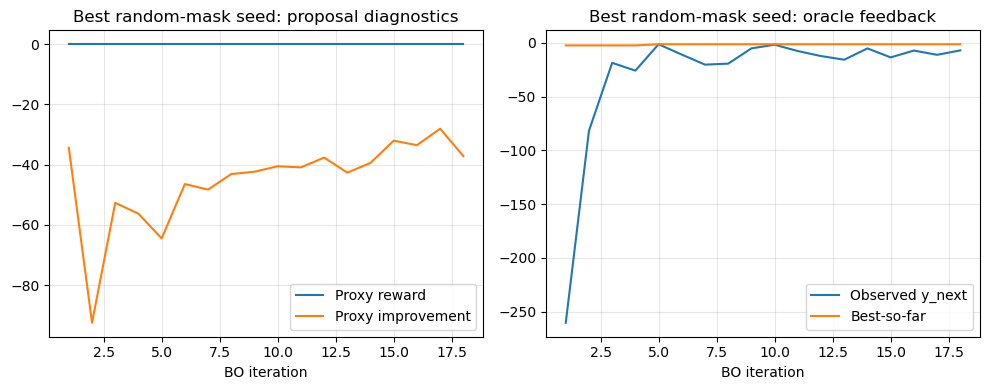
\includegraphics[width=\textwidth]{img/branin_random_diagnostics.png}
        \caption{Best random-mask seed on Branin}
    \end{subfigure}
    \hfill
    \begin{subfigure}[t]{0.48\textwidth}
        \centering
        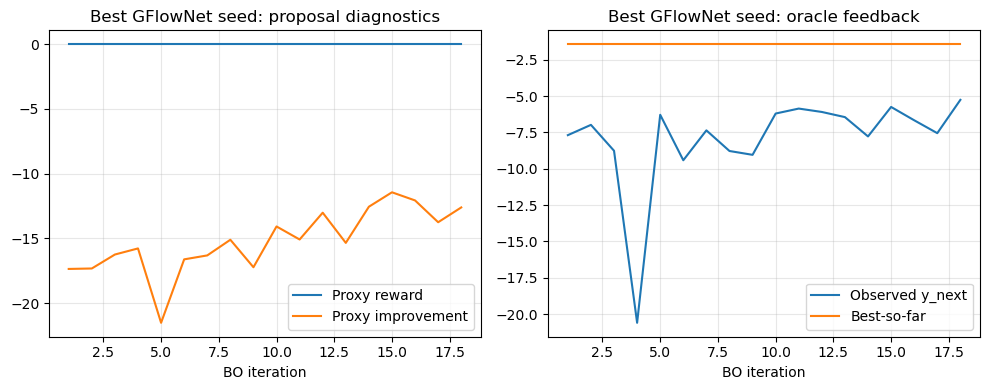
\includegraphics[width=\textwidth]{img/branin_gfn_diagnostics.png}
        \caption{Best GFlowNet seed on Branin}
    \end{subfigure}
    \caption{Branin proposal diagnostics. The random baseline still converts sampled proposals into a better final best-so-far value than the learned policy, despite the GFlowNet run being somewhat more consistent across seeds.}
    \label{fig:branin_diagnostics_appendix}
\end{figure*}

\begin{figure*}[t]
    \centering
    \begin{subfigure}[t]{0.48\textwidth}
        \centering
        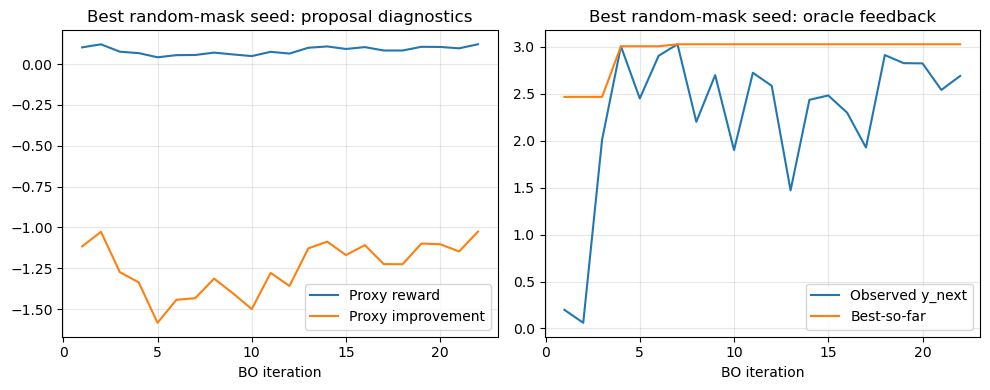
\includegraphics[width=\textwidth]{img/hartmann6_random_diagnostics.png}
        \caption{Best random-mask seed on Hartmann-6}
    \end{subfigure}
    \hfill
    \begin{subfigure}[t]{0.48\textwidth}
        \centering
        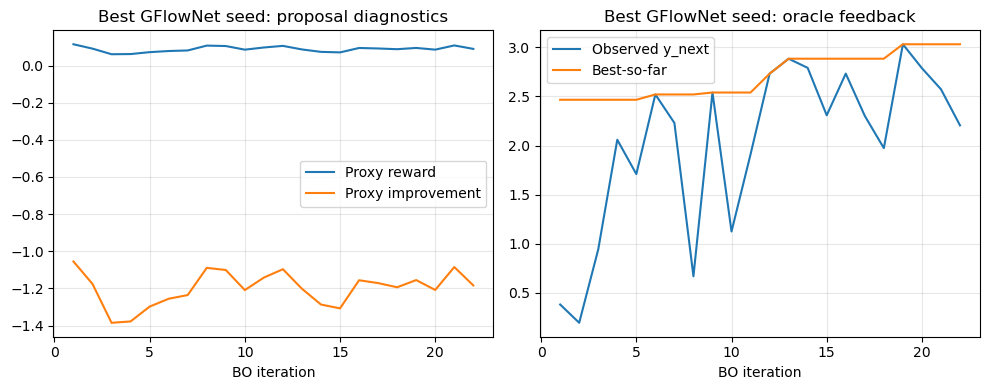
\includegraphics[width=\textwidth]{img/hartmann6_gfn_diagnostics.png}
        \caption{Best GFlowNet seed on Hartmann-6}
    \end{subfigure}
    \caption{Hartmann-6 proposal diagnostics. The learned policy remains viable, but its proxy-driven proposals do not translate into lower final regret than random mask sampling in this benchmark.}
    \label{fig:hartmann_diagnostics_appendix}
\end{figure*}

\bibliographystyle{plainnat}
\bibliography{references}

\end{document}
